% reset section counter
%\setcounter{section}{0}

%\metadata{lecture ID}{Your names}{date}
\metadata{12}{Rohan Taori and Jonathan Lee}{Feb 24nd, 2021}

\sec{Neural tangent kernel (NTK) approach}
In general, the loss landscapes of neural networks (with nonlinearities) is currently not as well understood. We now introduce the \textit{neural tangent kernel} which allows us to make some characterizations of the loss near a given neural network initialization.

\begin{figure}
    \centering
    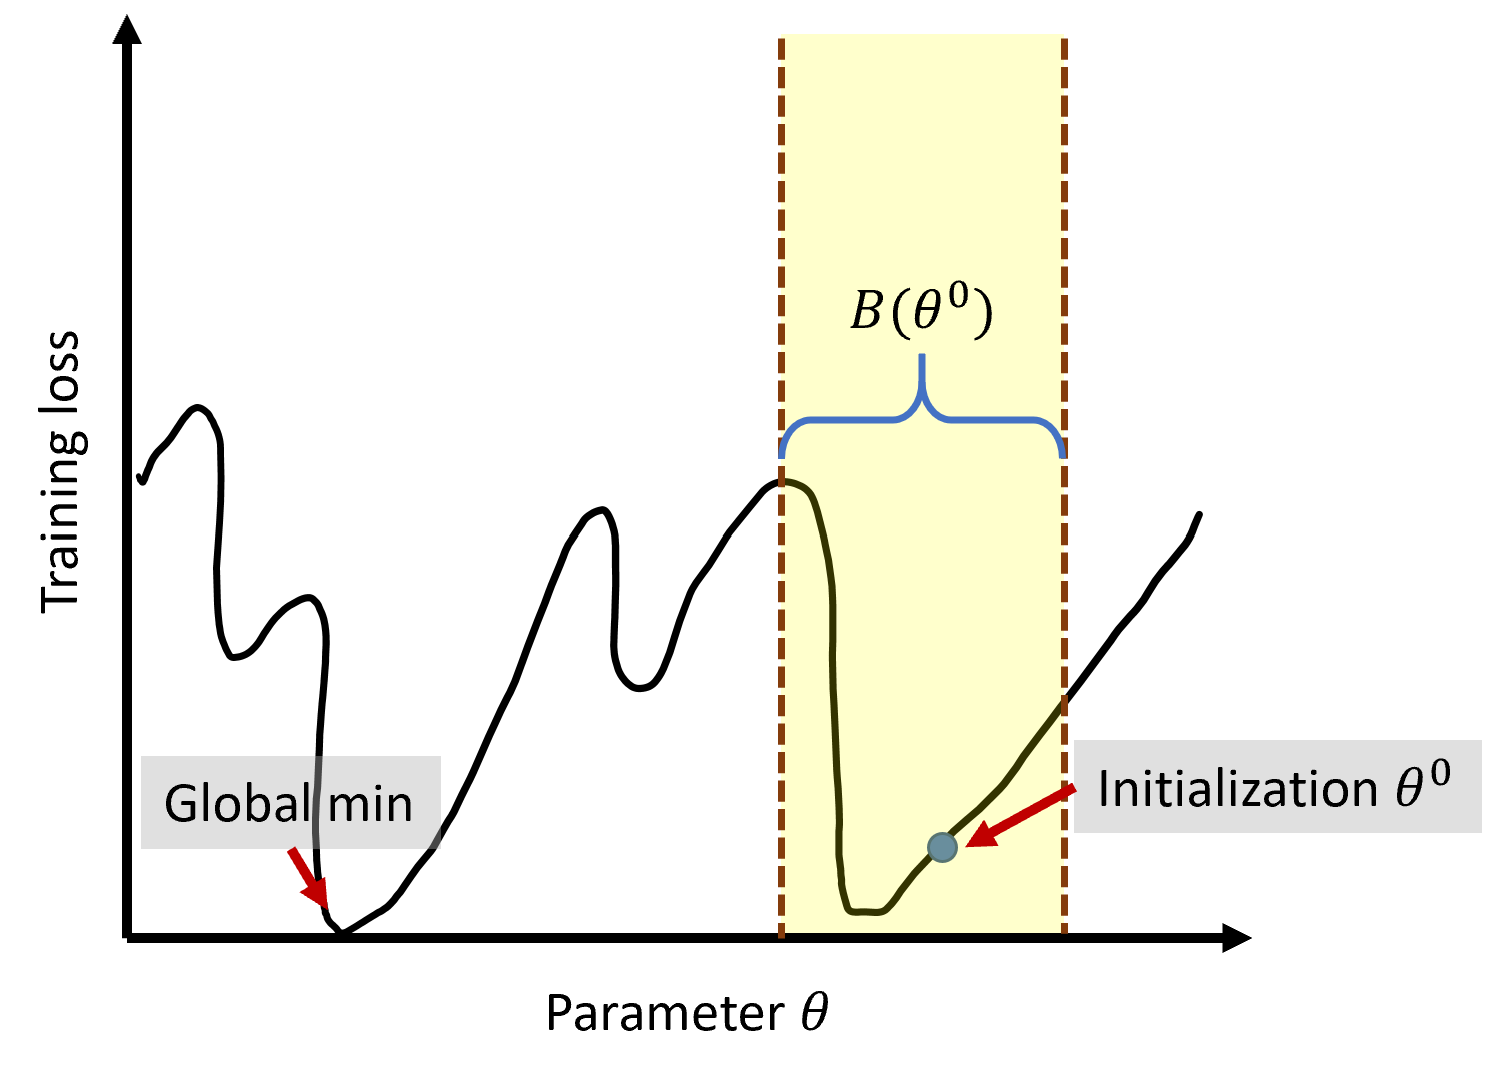
\includegraphics[width=2.5in]{figures/ntk-loss-landscape.png}
    \caption{The training loss landscape around a given parameter initialization $\theta^0$. We hope that the neighborhood around $\theta^0$ contains a local minimum that is close to the global minimum.}
    \label{lec11:fig:ntk_loss_landscape}
\end{figure}

The key insight of the NTK approach is that if we take an appropriate random parameter initialization $\theta^0$ (which we will choose later), we can identify a special neighborhood of $\theta^0$, denoted $B(\theta^0)$, where ``everything is nice''. That is, the function is convex in $B(\theta^0)$, there is a global minimum in the $B(\theta^0)$, and the algorithm starting at $\theta^0$ will converge to that global minimum. (See Figure~\ref{lec11:fig:ntk_loss_landscape} for an illustration.)

Take a random initialization $\theta = \theta^0$ and Taylor expand the loss around $\theta^0$ w.r.t. $\theta$:
\begin{align}
f_\theta(x) &= \underbrace{f_{\theta^0}(x) + \langle \nabla_\theta f_{\theta^0}(x), \theta - \theta^0 \rangle}_{g_\theta(x)} + O((\theta-\theta^0)^2).
\end{align}

In other words, we take the tangent plane to $f_\theta$ at $x$ (a linear approximation). We observe that $g_\theta$ is an affine function of $\theta$. Additionally, defining $\Delta \theta = \theta - \theta^0$, we see that the first term does not depend on $\Delta \theta$ while the second term $\langle \nabla_\theta f_{\theta^0}(x), \theta - \theta^0 \rangle$ is linear in $\Delta \theta$. (For convenience, we will sometimes choose to design $\theta^0$ such that $f_{\theta^0}(x) = 0$ so that $g_\theta$ is linear in $\theta^0$. However, the difference is not very important since $f_{\theta^0}(x)$ can simply be subsumed in the training labels $y$ via $y' = y - f_{\theta^0}(x)$.)

Now we have that $y \approx \nabla_\theta f_{\theta^0}(x)^\top \Delta \theta$. We can view $\phi(x) \triangleq \nabla_\theta f_{\theta^0}(x)$ as a feature map, i.e. we can rewrite the expression as $\phi(x)^\top \Delta \theta$ where $\phi(x)$ is fixed (only depends on $\theta^0$ and the architecture). This observation motivates the definition of the \textit{neural tangent kernel}:

\begin{definition}[Neural tangent kernel]
The \emph{neural tangent kernel} $K$ is defined as the function
\begin{equation}
K(x, x') = \langle \phi(x), \phi(x')\rangle = \langle \nabla f_{\theta^0}(x), \nabla f_{\theta^0}(x') \rangle.
\end{equation}
\end{definition}

Suppose we fit $g_\theta(x)$ to $y$, i.e. we minimize the loss 
\begin{equation}
\textrm{Loss} = \ell(\phi(x)^\top \Delta \theta, y),
\end{equation}
where $\phi(x)^\top\Delta \theta$ is linear and the loss as a whole is convex.
We will show that for a sufficiently wide neural network with proper initialization $\theta^0$, optimizing $f_\theta(x)$ starting from $\theta^0$ never leaves the neighborhood of $\theta^0$, effectively behaving the same as optimizing $g_\theta(x)$. In particular, two questions have to be answered:

\begin{enumerate}
    \item \textit{Why does there exist a small neighborhood $B(\theta^0)$ such that there exists a global minimum in $B(\theta^0)$?} This is more surprising, and it involves proper design of $\theta^0$. We will spend the rest of this chapter answering this question mathematically.
    \item \textit{Does gradient descent on the original loss with respect to $f_\theta(x)$ stay in the neighborhood $B(\theta^0)$?} The answer to this question is ``yes''. However, more technical machinery is required to prove it. We skip discussion of this as it is the less surprising claim.
\end{enumerate}

\subsec{The two-layer network case}

We demonstrate the NTK approach for the two-layer network setup. For $i \in [m]$, let $a_i \in \R$ be scalars and let $w_i \in \R^d$ be vectors. Let $\sigma: \R \to \R$ be the ReLU activation function defined as $\sigma(t) = \max\{ t, 0\}$. Suppose we have the following two-layer network:
\begin{equation}\label{lec12:eqn:network}
\hat{y} = f_\theta(x) = \frac{1}{\sqrt{m}} \sum_{i=1}^m a_i \sigma (w_i^\top x),
\end{equation}
for some input $x$.

Our weight matrix is $W = \begin{bmatrix} w_1^\top \\ \vdots \\ w_m^\top \end{bmatrix} \in \R^{m \times d}$. We initialize $W$ randomly using $W_{ij} \stackrel{i.i.d.}{\sim} \mathcal{N}(0, 1)$ for all $i$ and $j$. We initialize $a_i \in \{\pm 1\}$ and assume that the $a_i$'s are fixed after initialization, i.e. not updated during training. (We fix $a_i$ for simplicity: the results still hold when we are allowed to optimize $a_i$ in training.) We also assume that $x$ has norm on the order of $1$, and that the true label $y$ is on the order of $1$.

In our analysis, we will assume we have sufficiently large $m = \poly(n, d)$. In other words, the width of the network $m$ is sufficiently large such that $\poly(n, d)$ factors are not important in the analysis. For simplicity, we write $O_{d,n}(1)$ to hide polynomial dependencies on $d$ and $n$. Thus $O_{d,n}(m^c) = m^c \cdot \poly(n, d)$.

\textbf{Why do we need the scaling factor $1 / \sqrt{m}$ in Equation~\eqref{lec12:eqn:network}?} It is included to prevent the model outputs from blowing up when we increase the number of neurons $m$. Note that $\sigma (w_i^\top x) \approx O_{d,n}(1)$ since $w_i^\top \approx O_{d,n}(1)$ and $x \approx O_{d,n}(1)$. Since $a_i \in \{ \pm 1\}$ for all $i$, this implies that $ \sum_{i=1}^m a_i \sigma (w_i^\top x) \approx O_{d,n}(\sqrt{m})$. Thus, the scaling factor is needed to obtain $\hat{y} = f_\theta(x) = O_{d,n}(1)$.

Next, we introduce some notation that will be helpful for our analysis. Let $\Delta \theta = \theta - \thetazero$. Suppose we have $n$ examples $x^{(1)},...,x^{(n)}$ and labels $y^{(1)},...,y^{(n)}$. Let $\vec{y} = \begin{bmatrix} y^{(1)} & \dots & y^{(n)} \end{bmatrix}^\top$. Let
\begin{equation}
\vec{y'} = \begin{bmatrix} y^{(1)}-f_{\thetazero}(x^{(1)}) \\ \vdots \\ y^{(n)}-f_{\thetazero}(x^{(n)}) \end{bmatrix}
\end{equation}
be the transformed labels where we subsume the affine term in the label, allowing us to treat this as a purely linear model without loss of generality. Note that $\theta = \text{vec}(W) \in \R^{dm}$ is the vectorized version of the weights. Let $\Phi^{(i)} = \nabla_\theta f_{\thetazero}(x^{(i)}) \in R^{dm}$ be the feature associated with the $i$th example, and let $\Phi$ denote the collection of the features across the examples:
\begin{equation}
\Phi = \begin{bmatrix} \Phi^{(1)^\top} \\ \vdots \\ \Phi^{(n)^\top} \end{bmatrix} \in R^{n \times dm}.
\end{equation}

Recall that we defined
\begin{align}
    g_\theta(x) = f_{\thetazero}(x) + \langle\nabla_\theta f_{\thetazero}, \theta - \thetazero\rangle,
\end{align}
which is the linear approximation of $f_\theta(x)$ at $\thetazero$. If we wish to fit $g_\theta(x)$ to $y$ with the $\ell_2$-loss, we may consider minimizing the following objective function over $\theta$:
\begin{align}
\sum_{i=1}^n \left( y^{(i)} - f_{\thetazero}(x^{(i)}) - \langle \nabla_\theta f_{\thetazero}(x\sp{i}), \theta - \thetazero \rangle \right)^2 
&=  \sum_{i=1}^n \left(y^{(i)} - f_{\thetazero}(x^{(i)}) - \Delta\theta^\top \Phi^{(i)} \right)^2 \\
&=  \norm{\vec{y'} - \Phi \Delta\theta}_2^2.
\end{align}
This is equivalent to the following optimization problem:
\begin{align}
    \min_{\Delta \theta} \quad \norm{\vec{y'} - \Phi \Delta\theta}_2^2. \label{lec12:eqn:opt-problem}
\end{align}
Since $n \ll dm$, so we have an undetermined linear system. Since our goal is to show that the relevant neighborhood around $\thetazero$ is small, we should choose the minimum norm solution which can be found directly by the pseudoinverse: $\hat{\theta} = \Phi^+ \vec{y'}$,  where $\Phi^+$ is the pseudoinverse of $\Phi$ given by $\Phi^+ = \Phi^\top (\Phi \Phi^\top)^{-1}$.

It remains to show that the norm of $\hat{\theta}$ is small. Before we can do that, we will prove some useful claims:

\begin{lemma}[$\Phi$ is a well-conditioned matrix]\label{lec12:lem:claim1}
When $\thetazero$ is random, $\Phi$ is well-conditioned in the sense that \begin{align}
\sigma_{\min}(\Phi) \approx \frac{1}{\sqrt{n}} \norm{\Phi}_F \quad \text{and} \quad
\sigma_{\max}(\Phi) \approx \frac{1}{\sqrt{n}} \norm{\Phi}_F.
\end{align}
($\sigma_{\min}(\Phi)$ and $\sigma_{\max}(\Phi)$ denote the smallest and largest singular values of $\Phi$ respectively.) Specifically, $\sigma_{min}(\Phi) \gtrsim \Omega \left( \frac{1}{\sqrt{n}} \norm{\Phi}_F \right)$, and vice-versa for $\sigma_{\max}(\Phi)$.
{\color{blue} Note: this lemma is very problematic and perhaps outright wrong. It will be updated in the next revision} \tnoteimp{Tengyu will fix this}
\end{lemma}

We omit the proof as it uses tools from random matrix theory that are not required for this course. (The high-level idea is to show that $\Phi \Phi^\top \approx c \cdot I$ for some constant scalar $c$.)

\begin{remark}
Since $\Phi \in R^{n \times dm}$, $\Phi$ has at most $n$ singular values $\sigma_1 \geq \ldots \geq \sigma_n \geq 0$. Since $\norm{\Phi}_F = \sqrt{\sigma_1^2 + ... + \sigma_n^2}$, the fact that $\sigma_n \approx \frac{1}{\sqrt{n}} \norm{\Phi}_F$ means that all the singular values are not very different from each other.
\end{remark}

\begin{lemma}[Frobenius norm of $\Phi$ is order $1$]\label{lec12:lem:phi-norm}
$\norm{\Phi}_F \asymp \Theta_{d,n}(1)$, which implies that
\begin{equation}
\norm{\Phi}_{\text{op}}, \ \norm{\Phi^+}_{\text{op}}  \asymp \Theta_{d,n}(1).
\end{equation}
\end{lemma}

\begin{proof}
Applying the definition of $\Phi^{(i)}$, we have 
\begin{align}
    \Phi^{(i)} &= \text{vec}\left(\frac{\partial f_{\theta}(x^{(i)})}{\partial W}\right) = \frac{1}{\sqrt{m}} (a \odot \sigma' (w x^{(i)})) \cdot \left(x^{(i)}\right)^\top.
\end{align}

Thus, its norm can be written as
\begin{align}
\norm{\Phi^{(i)}}_2 &= \frac{1}{\sqrt{m}} \norm{a \odot \sigma' (w x^{(i)})}_2 \cdot \norm{x^{(i)}}_2  \\
&\approx \Theta_{d,n}\left(\frac{1}{\sqrt{m}} \cdot \sqrt{m} \cdot 1 \right) \label{lec12:eqn:approx} \\
&\approx \Theta_{d,n}(1).
\end{align}
The first equality is because $\norm{ab^\top}_2 = \norm{a}_2 \cdot \norm{b}_2 / \norm{ab^\top}_F$ for any vectors $a$ and $b$, and \eqref{lec12:eqn:approx} is because $\norm{x^{(i)}}_2$ is on order of $1$, $a \odot \sigma' (w x^{(i)})$ is a vector of length $m$ with each entry being on the order of $1$ (each $a_i$ is either $1$ or $-1$, and $\sigma'$ is either $0$ or $1$). Summing up over the $\Phi^{(i)}$'s,
\begin{align}
\norm{\Phi}_F &= \sqrt{\sum_{i=1}^n \norm{\Phi^{(i)}}_2^2} \approx \Theta_{d,n}(1).
\end{align}

Putting this together with Lemma~\ref{lec12:lem:claim1}, all the singular values of $\Phi$ are $\Theta_{d,n}(1)$. By extension,  $\norm{\Phi^+}_{\text{op}} \asymp \Theta_{d,n}(1)$ as well, since if a matrix $A$ has singular values $\sigma_1, \dots,\sigma_n$, $A^+$ has singular values $1 / \sigma_1, \dots,1/\sigma_n$. 
\end{proof}

Now we can leverage the previous two lemmas to produce a bound on the $\ell_2$-norm of the solution of the optimization problem~\eqref{lec12:eqn:opt-problem}, $\hat \theta$. Recall that $\hat \theta = \Phi^+ \vec {y'}$. Upper bounding the norm yields
\begin{align}
    \| \hat \theta\|_2 & \leq \| \Phi^+ \|_{\text{op}} \cdot \|\vec{y'} \|_2  \\
    & \leq O_{d, n} (1) \cdot \|\vec{y'} \|_2 &\text{(by Lemma~\ref{lec12:lem:phi-norm})} \\
    & \leq  O_{d, n} (1),
\end{align}
where the last inequality is because $\vec{y'}$ is of dimension $n$ and each entry is on the order of $1$ (the original labels are on the order of $1$ and the shifts $f_{\thetazero}(x\sp{i})$ are also on the order of $1$). Although $\| \hat \theta\|_2$ may not appear to be small, since it may still be $\poly(d, n)$, we can view it as comparatively small relative to the size of $\thetazero$ since
\begin{align}
    \| \thetazero \|_2 &= \| W^0 \|_F^2 \\
    &\asymp \sqrt {dm} &\text{(because $ W^0$ has $dm$ entries of order $1$)} \\
    &= \Theta_{d, n}(\sqrt m).
\end{align}
Thus, the neighborhood size is much smaller than the norm of the initialization in terms of $m$. Further justification of the $\ell_2$-norm as a reasonable metric for defining neighborhood size may require deeper inspection of the higher order terms and their behavior within the neighborhood. The intuition is that one only needs to move a little to reach the solution. Relative to the norm of the initialization, the neighborhood size is shrinking.

\begin{remark}
While we do not cover this in detail, the main takeaway on the optimization front is that the problem of fitting $g_\theta(x)$ is a standard strongly convex optimization problem, which enjoys the geometric rate of convergence.
\end{remark}



